% ============================================================
% Diagram: Data Linking and Dataset Building Procedure
% Compile with: pdflatex diagram_data_pipeline.tex
% Requires: tikz, tikzlibrary{shapes,arrows.meta,positioning,fit,backgrounds,calc}
% ============================================================
\documentclass[tikz, border=12pt]{standalone}
\usepackage{tikz}
\usepackage{xcolor}
\usetikzlibrary{shapes.geometric, arrows.meta, positioning, fit, backgrounds, calc}

% ── Colour palette ────────────────────────────────────────────────────────────
\definecolor{srcblue}{RGB}{210,228,255}
\definecolor{srcblueborder}{RGB}{60,100,180}
\definecolor{crosswalkpurp}{RGB}{230,215,255}
\definecolor{crosswalkborder}{RGB}{110,60,180}
\definecolor{procamber}{RGB}{255,235,200}
\definecolor{procborder}{RGB}{200,120,20}
\definecolor{matchgreen}{RGB}{210,240,220}
\definecolor{matchborder}{RGB}{40,130,70}
\definecolor{finalred}{RGB}{255,220,215}
\definecolor{finalborder}{RGB}{180,50,40}
\definecolor{annotgrey}{RGB}{100,100,100}

% ── Node styles ───────────────────────────────────────────────────────────────
\tikzset{
  srcbox/.style  = {draw=srcblueborder,   fill=srcblue,      rounded corners=4pt,
                    text width=3.4cm, align=center, font=\small,
                    inner sep=6pt, minimum height=1.0cm},
  crossbox/.style= {draw=crosswalkborder, fill=crosswalkpurp, rounded corners=4pt,
                    text width=3.6cm, align=center, font=\small,
                    inner sep=6pt, minimum height=1.0cm},
  procbox/.style = {draw=procborder,      fill=procamber,     rounded corners=4pt,
                    text width=4.0cm, align=center, font=\small,
                    inner sep=6pt, minimum height=1.0cm},
  matchbox/.style= {draw=matchborder,     fill=matchgreen,    rounded corners=4pt,
                    text width=4.2cm, align=center, font=\small,
                    inner sep=6pt, minimum height=1.0cm},
  finalbox/.style= {draw=finalborder,     fill=finalred,      rounded corners=6pt,
                    text width=10cm, align=center, font=\small\bfseries,
                    inner sep=8pt, minimum height=1.2cm},
  stepbox/.style = {draw=procborder,      fill=procamber,     rounded corners=4pt,
                    text width=8.0cm, align=center, font=\small,
                    inner sep=6pt, minimum height=1.0cm},
  arrow/.style   = {-{Latex[length=2.5mm]}, thick, color=black!60},
  thinnarrow/.style = {-{Latex[length=2mm]}, semithick, color=black!50},
  annot/.style   = {font=\footnotesize\itshape, color=annotgrey, align=center},
  legend/.style  = {draw=black!30, fill=white, rounded corners=3pt,
                    inner sep=6pt, font=\footnotesize}
}

\begin{document}
\begin{tikzpicture}[node distance=0.55cm and 0.5cm]

% ══════════════════════════════════════════════════════════════════════════════
% ROW 1 — Raw source files
% ══════════════════════════════════════════════════════════════════════════════
\node[srcbox] (nrega) {%
  \textbf{\texttt{nrega.dta}}\\[2pt]
  Kjelsrud replication\\
  151{,}660 GP-years\\
  (treatment, controls, FE)};

\node[srcbox, right=0.7cm of nrega] (gpnames) {%
  \textbf{\texttt{gp\_id\_names.dta}}\\[2pt]
  GP name strings\\
  for name-matching\\
  151{,}660 GPs};

\node[srcbox, right=0.7cm of gpnames] (mis) {%
  \textbf{\texttt{mis\_avg\_sc\_st\_data.csv}}\\[2pt]
  Mittal SC/ST person-days\\
  (numerator of\\
  targeting ratio)};

\node[srcbox, right=0.7cm of mis] (pancat) {%
  \textbf{\texttt{panchayat\_category.csv}}\\[2pt]
  Mittal SC/ST population\\
  (denominator of\\
  targeting ratio)};

% ══════════════════════════════════════════════════════════════════════════════
% ROW 2 — SHRUG crosswalk (feeds into name-matching)
% ══════════════════════════════════════════════════════════════════════════════
\node[crossbox, below=1.1cm of gpnames, xshift=0.5cm] (shrug) {%
  \textbf{SHRUG Crosswalk}\\[2pt]
  \texttt{pc11r\_shrid\_key.csv}\\
  + \texttt{shrid\_loc\_names.csv}\\
  Numeric codes $\to$ state \&\\
  district name strings};

% Arrow: gpnames -> shrug
\draw[arrow] (gpnames.south) -- ++(0,-0.38) -| (shrug.north);

% ══════════════════════════════════════════════════════════════════════════════
% ROW 3 — Processing: collapse + name-match x2
% ══════════════════════════════════════════════════════════════════════════════
\node[procbox, below=1.1cm of nrega] (collapse) {%
  \textbf{Collapse to GP level}\\[2pt]
  Drop duplicate years;\\
  keep time-invariant covariates\\
  \textit{150{,}413 unique GPs}};

\node[matchbox, right=0.6cm of collapse, xshift=1.0cm] (match1) {%
  \textbf{3-key name match}\\[2pt]
  (state, district, GP name)\\
  exact match after cleaning\\
  \textit{$\approx$119K matched (79\%)}\\
  Duplicates: keep max person-days};

\node[matchbox, right=0.65cm of match1] (match2) {%
  \textbf{3-key name match}\\[2pt]
  (state, district, GP name)\\
  exact match after cleaning\\
  \textit{$\approx$65K matched (43\%)}\\
  \textbf{Binding constraint}};

% Arrows into row 3
\draw[arrow] (nrega.south)   -- (collapse.north);
\draw[arrow] (shrug.south)   -- ++(0,-0.3) -| (match1.north);
\draw[arrow] (mis.south)     -- (match1.north);
\draw[arrow] (shrug.south)   -- ++(0,-0.3) -| (match2.north);
\draw[arrow] (pancat.south)  -- (match2.north);

% Annotation: match rates
\node[annot, right=0.1cm of match1, yshift=0.15cm] {\textit{79\%}};
\node[annot, right=0.1cm of match2, yshift=0.15cm] {\textit{43\%}};

% ══════════════════════════════════════════════════════════════════════════════
% ROW 4 — Left-merge everything onto nrega frame
% ══════════════════════════════════════════════════════════════════════════════
\node[stepbox, below=1.1cm of match1, xshift=-0.5cm] (merge) {%
  \textbf{Left-merge all sources onto \texttt{nrega} frame}\\[2pt]
  Join on \texttt{gp\_id} (Kjelsrud internal GP identifier)\\
  Unmatched GPs retain \texttt{NaN} for Mittal-derived columns};

% Arrows into merge
\draw[arrow] (collapse.south) -- ++(0,-0.35) -| (merge.west);
\draw[arrow] (match1.south)   -- (merge.north);
\draw[arrow] (match2.south)   -- ++(0,-0.35) -| (merge.east);

% ══════════════════════════════════════════════════════════════════════════════
% ROW 5 — Construct targeting ratios
% ══════════════════════════════════════════════════════════════════════════════
\node[stepbox, below=0.6cm of merge] (ratios) {%
  \textbf{Construct targeting ratios (SC, ST, SC+ST)}\\[2pt]
  $\text{TargetingRatio}(G,j) =
  \dfrac{\text{person-days share of group }G}{\text{population share of group }G}$
  \quad Winsorise [1st, 99th pct] $\to$ log-transform};

\draw[arrow] (merge.south) -- (ratios.north);

% ══════════════════════════════════════════════════════════════════════════════
% ROW 6 — Standardise treatment + sample restrictions
% ══════════════════════════════════════════════════════════════════════════════
\node[stepbox, below=0.6cm of ratios] (restrict) {%
  \textbf{Standardise treatment \& apply sample restrictions}\\[2pt]
  Standardise \texttt{fragmentation\_2004\_past} to zero mean, unit SD\\
  Keep: non-missing treatment + \texttt{pc\_dist} FE cell + all 9 controls + $\geq$1 outcome};

\draw[arrow] (ratios.south) -- (restrict.north);

% ══════════════════════════════════════════════════════════════════════════════
% ROW 7 — Final dataset
% ══════════════════════════════════════════════════════════════════════════════
\node[finalbox, below=0.6cm of restrict] (final) {%
  \textbf{Final Analysis Dataset:}\ \texttt{gp\_analysis\_dataset.csv}\\[3pt]
  \textbf{47{,}995 GPs} $\times$ \textbf{33 columns} $\quad|\quad$ 14 states\\[2pt]
  SC regression: 44{,}915 GPs \quad ST regression: 18{,}563 GPs (ST pop $\geq$ 5\%)
  \quad SC+ST: 47{,}995 GPs};

\draw[arrow] (restrict.south) -- (final.north);

% ══════════════════════════════════════════════════════════════════════════════
% Background panel — source files
% ══════════════════════════════════════════════════════════════════════════════
\begin{pgfonlayer}{background}
  \node[draw=srcblueborder!60, fill=srcblue!20, rounded corners=6pt,
        fit=(nrega)(pancat), inner sep=8pt,
        label={[font=\footnotesize\bfseries\color{srcblueborder}]above:Raw Source Files}] {};
\end{pgfonlayer}

% ══════════════════════════════════════════════════════════════════════════════
% Legend
% ══════════════════════════════════════════════════════════════════════════════
\node[legend, below=0.8cm of final, xshift=-3cm] (leg) {%
  \begin{tabular}{cl}
  \tikz\node[srcbox,  text width=0.5cm, minimum height=0.35cm, inner sep=2pt]{}; &
    Raw source file \\[3pt]
  \tikz\node[crossbox,text width=0.5cm, minimum height=0.35cm, inner sep=2pt]{}; &
    Crosswalk / lookup \\[3pt]
  \tikz\node[matchbox, text width=0.5cm, minimum height=0.35cm, inner sep=2pt]{}; &
    Name-matching step \\[3pt]
  \tikz\node[procbox,  text width=0.5cm, minimum height=0.35cm, inner sep=2pt]{}; &
    Processing / aggregation \\[3pt]
  \tikz\node[finalbox, text width=0.5cm, minimum height=0.35cm, inner sep=2pt]{}; &
    Final analysis dataset \\
  \end{tabular}};

\end{tikzpicture}
\end{document}
